\documentclass[tikz,border=2mm]{standalone}
\usepackage{amssymb}
\usepackage{pgfplots}
\usetikzlibrary[arrows.meta]
\usetikzlibrary{positioning, shapes, calc}

\tikzset{set/.style={draw,circle,inner sep=0pt,align=center}}
\tikzset{line/.style = {draw,thick, shorten >=-2pt, shorten <=-2pt}}
\tikzset{tick/.style={draw, minimum width=0pt, minimum height=2pt, inner sep=0pt, label=below:$#1$},tick/.default={}}
\begin{document}
	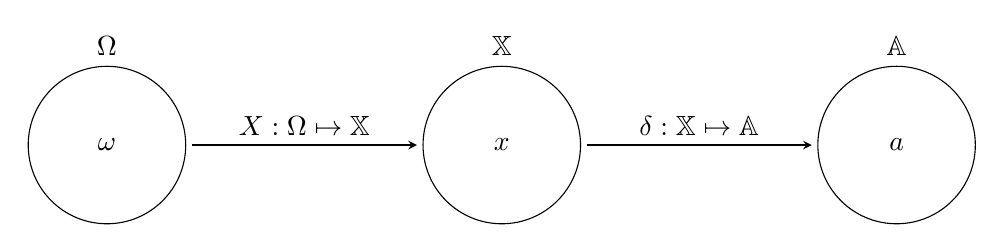
\begin{tikzpicture}[
		node distance=2cm,
		set/.style={draw, circle, minimum size=2cm},
		randomvar/.style={draw, rectangle, minimum size=1.5cm},
		arrow/.style={->, >=stealth, shorten >=2pt, shorten <=2pt}
		]
		% Sample Space Omega
		
		\node[set, label={above:$\Omega$}] (omega) {$\omega$};
		\node[set, right= 3cm of omega, label={above:$\mathbb{X}$}] (X) {$x$};
		\node[set, right= 3cm of X, label={above:$\mathbb{A}$}] (A) {$a$};

		\draw[arrow] (omega) -- node[above] {$X: \Omega \mapsto \mathbb{X}$} (X);
		\draw[arrow] (X) -- node[above] {$\delta: \mathbb{X} \mapsto \mathbb{A}$} (A);
		
	\end{tikzpicture}
	
	
	\begin{tikzpicture}[
		node distance=2cm,
		set/.style={draw, circle, minimum size=2cm},
		randomvar/.style={draw, rectangle, minimum size=1.5cm},
		arrow/.style={->, >=stealth, shorten >=2pt, shorten <=2pt}
		]
		% Sample Space Omega
		\coordinate (c1) at (7,0);
		
		\node[set, label={above:$\Omega$}] (omega) {$\omega$};
		\node[set, right=of omega, label={above:$\mathbb{X}$}] (X) {x};
		\node[set, below= of c1, label={left:$\mathbb{A}$}] (A) {$a$};
		\node[set, above=of X, label={above:$\mathbb{Y}$}] (Y) {y};
		
		\node[set, below=of omega, label={left:$\mathcal{F}$}] (F) {$\sim 2^\Omega$};
		\node[right = of F] (unit) {$[0,1]$};
		
		\node[set, above = of c1, label={above:$\mathcal{P}$}] (P) {$P_w$};		
		\node[set, above = of Y, label={above:$\mathbb{W}$}] (G) {$w$};
		\node[set, left = of G, label={above:$\Gamma$}] (gamma) {$\gamma$};
		
		
		\node[right = 4cm of c1] (R) {$\mathbb{R}_{\geq 0}$};
		
		\draw[arrow] (gamma) -- node[above] {$W: \Gamma \mapsto \mathbb{W}$} (G);
		
		\draw (X) -- (c1);
		\draw (Y) -- (c1);
		\draw (G) -- (c1);
		\draw (P) -- (c1);
		\draw (A) -- (c1);
		
		\draw[arrow] (F) -- node[below] {$\mathbb{P}: \mathcal{F} \mapsto [0,1]$} (unit);
		\draw[arrow] (c1) -- node[above] {$C: \mathbb{X}\times \mathbb{Y}\times \mathbb{W}\times \mathbb{A} \mapsto \mathbb{R}$} (R);
		\draw[arrow] (omega) -- node[above] {} (F);
		\draw[arrow] (omega) -- node[above] {$X: \Omega \mapsto \mathbb{X}$} (X);
		\draw[arrow] (omega) -- node[left] {$Y: \Omega \mapsto \mathbb{Y}$} (Y);
		
		\draw[dashed] (0,8) ellipse (3 and 1.5);
		
		% Add text above the oval
		\node[above] at (0,5.5) {Bayesian addition};
		
	\end{tikzpicture}
	
\end{document}

